\documentclass[10pt]{article}
\usepackage{icmlko}

\icmlmeta{IP 파운데이션 월드모델}{18}{다섯은 실은 둘이었다}{축을 이름으로 맞추지 말고 인자로 맞춰라 --- 여섯 방향 중 다섯이 건너간다}

\begin{document}

\twocolumn[
\icmlheader

\begin{abstract}
노트 16이 가격을 입장 허들 자리에서 뺀 뒤 그 자리는 세 도메인 모두 비어 있었다.
게임에서 가격과 독립인 접근 장벽 --- 최소 사양, 연령 등급 --- 을 수집해 채워 봤다.
\textbf{전부 실패했다.} 최소 저장 공간 $+$0.393, 최소 RAM(동시대 대비) $+$0.284,
연령 등급 $+$0.255로 모두 양수이고, 규모와 폭과 가격을 통제해도 양수로 남는다
($+$0.347, $+$0.224, $+$0.223). 장벽처럼 보이는 모든 것이 규모 신호로 작동한다.
그래서 축을 하나씩 검정하는 대신 \textbf{구조를 직접 봤다}. 게임 원자료 8변수의
주성분 분석에서 두 인자가 나온다 --- PC1은 저장 공간·가격·RAM·연령이 모이는
\textbf{제작 규모}(37\%, 라벨과 $+$0.408), PC2는 기능 수·언어 수·플랫폼 수가
모이는 \textbf{도달 폭}(16\%, $+$0.130)이다. 팝업의 열 개 속성도 같은 구조다
(PC1 29\%, 라벨과 $+$0.319). 다만 팝업에서는 입장 허들이 PC2에 가장 강하게
실리고 라벨과 음의 관계다 --- \textbf{허들 축은 팝업에서 살아 있고 게임에서만
죽는다.} 그리고 실용적 결론이 따라온다. 각 도메인이 관측 가능한 축을 전부 써서
두 인자로 압축하면 \textbf{여섯 방향 중 다섯이 유의하게 전이된다}(명명 축은 넷).
효과 크기가 최대 두 배로 커지고, 노트 13이 세운 ``공유 슬롯 수는 관측 가능성의
교집합이 정한다''는 제약이 풀린다.
\end{abstract}
]

\section{허들을 다시 찾아 나섰다}

노트 16은 두 도메인에서 가격이 허들이 아니라 규모 신호임을 보이고 그 자리를 비웠다.
축 자체를 폐기한 것은 아니었다 --- ``닿는 데 무엇을 치르는가''는 실재할 수 있고
가격이 그것을 재지 못했을 뿐이다.

게임에는 가격과 독립인 장벽이 있다. \textbf{최소 사양}이다. 돈이 있어도 기기가
안 되면 못 산다. Steam이 주는 최소 사양 문자열에서 RAM과 저장 공간을 뽑고,
연령 등급도 함께 넣었다(482건 중 RAM 98\%, 저장 공간 94\% 파싱).

\paragraph{함정 하나는 미리 피했다}
사양을 절대값으로 쓰면 가격과 같은 함정에 빠진다 --- 사양이 높은 게임은 대개
대작이고, 사양 요구는 해가 갈수록 오른다(2015년의 8GB와 2026년의 8GB는 다른
뜻이다). 그래서 \emph{같은 해 출시작 대비} 상대값으로도 함께 쟀다.

\begin{figure}[t]
\centering
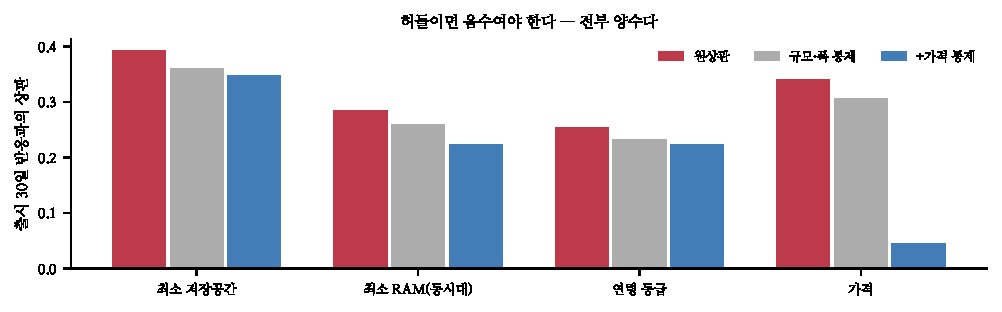
\includegraphics[width=\textwidth]{figs/friction.pdf}
\caption{장벽 후보와 출시 30일 반응의 관계. 허들이면 음수여야 한다.
규모와 폭을 통제해도 전부 양수다.}
\end{figure}

\begin{table}[t]
\centering\tsize
\caption{장벽 후보의 부분상관(n=336--434, 30일 창 라벨).}
\begin{tabular}{lrrr}
\toprule
후보 & 원상관 & 규모·폭 통제 & $+$가격 통제 \\
\midrule
최소 저장 공간 & $+$0.393 & $+$0.361 & $+$0.347 \\
최소 RAM (동시대 대비) & $+$0.284 & $+$0.259 & $+$0.224 \\
연령 등급 & $+$0.255 & $+$0.232 & $+$0.223 \\
가격 & $+$0.340 & $+$0.307 & $+$0.046 \\
\bottomrule
\end{tabular}
\end{table}

전부 실패했다. 동시대 대비 상대 사양까지 양수다. 하나 배운 것은 있다 ---
\textbf{가격은 사양을 통제하면 거의 사라진다}($+$0.307 $\to$ $+$0.046). 사양이
가격보다 근본적인 규모 지표다.

\claimx{게임 도메인에서 입장 허들 축은 관측되지 않는다. 가격·사양·연령 세 후보가
모두, 규모와 폭을 통제한 뒤에도 양의 관계다.}{규모 지표를 더 정교하게(개발사 인원,
개발 기간) 통제한 뒤 사양이 음의 관계로 돌아서면 축은 살아 있고 통제가 부족했던
것이다.}

\section{그래서 구조를 직접 봤다}

축을 하나씩 이름 붙여 검정하는 방식이 여기서 한계에 닿았다. 다른 질문을 던졌다 ---
\emph{이 변수들은 실제로 몇 개의 것인가.}

게임 원자료 8변수(언어 수, 장르 수, 플랫폼 수, 기능 수, 최소 RAM, 최소 저장 공간,
가격, 연령 등급)의 주성분 분석이다.

\begin{figure}[t]
\centering
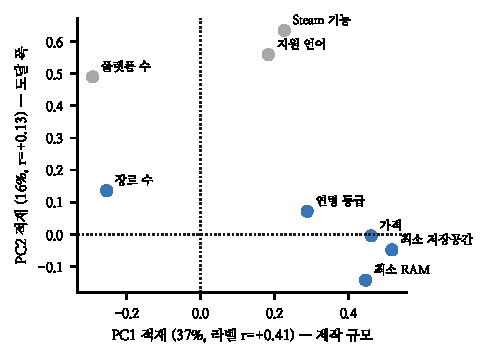
\includegraphics[width=\columnwidth]{figs/factors.pdf}
\caption{게임 원자료 8변수의 인자 적재. 오른쪽에 규모 지표가, 위쪽에 폭 지표가
모인다.}
\end{figure}

\begin{table}[t]
\centering\tsize
\caption{게임 원자료의 주성분(n=336).}
\begin{tabular}{llr}
\toprule
성분 & 주요 적재 & 라벨과 r \\
\midrule
PC1 (37\%) & 저장 공간 .52, 가격 .46, & \textbf{$+$0.408} \\
 & RAM .45, 연령 .29 & \\
PC2 (16\%) & 기능 수 .63, 언어 수 .56, & $+$0.130 \\
 & 플랫폼 수 .49 & \\
PC3 (12\%) & 장르 수 .77 & $+$0.061 \\
\bottomrule
\end{tabular}
\end{table}

두 인자가 나온다.

\begin{itemize}[leftmargin=1.1em,itemsep=0.15em]
\item \textbf{PC1 --- 제작 규모.} 얼마나 넣었는가. 내가 ``입장 허들''로 넣으려던
      것들(가격, RAM, 저장 공간, 연령)이 전부 여기 모인다. 별개 축이 아니라
      규모의 지표들이었다.
\item \textbf{PC2 --- 도달 폭.} 몇 명이 접근 가능한가. 언어 수와 플랫폼 수가
      모이는 것은 당연한데, 내가 ``굿즈 규모''로 쓴 Steam 기능 수도 여기 실린다.
\end{itemize}

\subsection{팝업도 같은 구조다 --- 한 가지만 빼고}

팝업의 열 개 서수 속성으로 같은 분석을 했다.

\begin{table}[t]
\centering\tsize
\caption{팝업 열 개 속성의 주성분(n=75).}
\begin{tabular}{llr}
\toprule
성분 & 주요 적재 & 라벨과 r \\
\midrule
PC1 (29\%) & 굿즈 .42, 포토존 .40, 콜라보 .37, & $+$0.319 \\
 & 미디어 .34, 매장 .32 & \\
PC2 (17\%) & \textbf{입장 허들 $+$.65}, 타깃 폭 $-$.56 & $-$0.240 \\
PC3 (12\%) & IP 인지 폭 .59, 시즌 적합 .49 & $-$0.182 \\
\bottomrule
\end{tabular}
\end{table}

PC1은 게임과 같다 --- 굿즈, 포토존, 콜라보, 미디어, 매장이 함께 움직이는
제작 규모다.

PC2가 다르다. \textbf{팝업에서는 입장 허들이 가장 강하게 실리고}(+0.65) 타깃 폭이
반대 방향으로 실린다($-$0.56). 즉 ``좁고 허들 높은'' 대 ``넓고 허들 낮은'' 축이며,
라벨과 음의 관계다($-$0.240) --- 좁히고 허들을 세우면 방문자가 준다.

\claimx{입장 허들 축은 팝업에서 살아 있고 게임에서만 죽는다. 팝업 PC2에 가장 강한
적재를 가지며 라벨과 음의 관계다. 축의 실재 여부는 도메인마다 다를 수 있다.}{팝업에서도
규모를 더 정교하게 통제하면 허들 적재가 사라지는 경우, 팝업 PC2는 허들이 아니라
규모의 반대편이었던 것이다.}

두 도메인의 PC2가 부호는 반대로 보이지만 같은 이야기다 --- 팝업 PC2는 ``좁힘''
방향이라 라벨과 음이고, 게임 PC2는 ``넓힘'' 방향이라 양이다. 둘 다 \emph{넓힐수록
좋다}를 말한다.

\section{그래서 인자로 전이한다}

여기서 실용적 귀결이 나온다. 노트 13은 이렇게 썼다.

\begin{quote}\fontsize{9.2}{11}\selectfont
공유 슬롯의 개수는 축의 개수가 아니라 관측 가능성의 교집합이 정한다.
\end{quote}

교집합은 둘이었다(타깃 폭, 굿즈 규모). 팝업은 다섯 축을 다 재는데도 게임이 두 개만
재므로 셋을 버려야 했다.

인자로 가면 그 제약이 풀린다. \textbf{도메인마다 관측 가능한 축을 전부 써서 각자
두 인자로 압축}하면 된다 --- 팝업 5개, 아이돌 3개, 게임 2개를 모두 쓰고, 결과는
같은 2차원이다.

\begin{figure}[t]
\centering
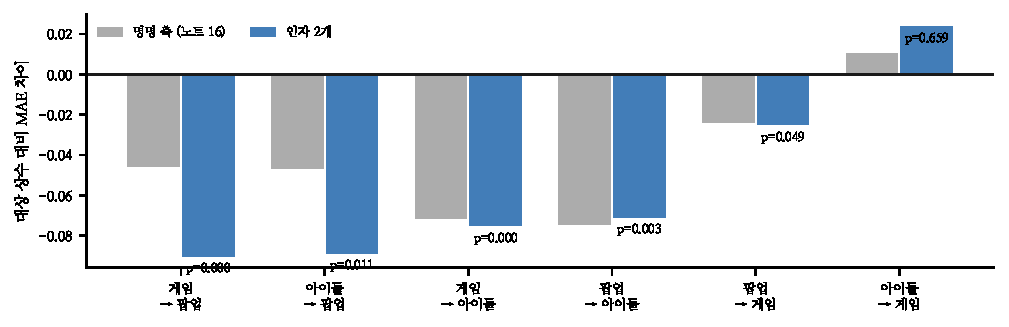
\includegraphics[width=\textwidth]{figs/pcvsnamed.pdf}
\caption{명명 축과 인자 표현의 전이 비교. 다섯 방향이 유의해지고 효과가 최대
두 배로 커진다.}
\end{figure}

\begin{table}[t]
\centering\tsize
\caption{전이 비교. 순열 3,000회, 대상 라벨 미사용.}
\begin{tabular}{lrrrr}
\toprule
방향 & \multicolumn{2}{c}{명명 축} & \multicolumn{2}{c}{인자 2개} \\
& 차이 & p & 차이 & p \\
\midrule
게임 $\to$ 팝업 & $-$0.0458 & 0.0003 & $-$0.0903 & \textbf{$<$0.0001} \\
아이돌 $\to$ 팝업 & $-$0.0467 & 0.0480 & $-$0.0888 & \textbf{0.0107} \\
게임 $\to$ 아이돌 & $-$0.0715 & $<$0.0001 & $-$0.0752 & \textbf{$<$0.0001} \\
팝업 $\to$ 아이돌 & $-$0.0744 & 0.0013 & $-$0.0712 & \textbf{0.0030} \\
팝업 $\to$ 게임 & $-$0.0239 & 0.0837 & $-$0.0251 & \textbf{0.0493} \\
\midrule
아이돌 $\to$ 게임 & $+$0.0104 & 0.4957 & $+$0.0238 & 0.6587 \\
\bottomrule
\end{tabular}
\end{table}

\textbf{여섯 중 다섯이 유의하다.} 명명 축에서는 넷이었다. 게임 $\to$ 팝업과
아이돌 $\to$ 팝업은 효과가 두 배로 커졌다.

\claimx{축을 이름으로 맞추는 것보다 인자로 맞추는 것이 낫다. 각 도메인이 관측
가능한 축을 전부 써서 두 인자로 압축하면 여섯 방향 중 다섯이 유의하게 전이되며,
공유 슬롯을 관측 가능성의 교집합으로 제한할 필요가 없다.}{네 번째 도메인에서
인자 구조가 다르게 나오면(예: PC1이 규모가 아닌 다른 것) 이 방식은 도메인이
늘수록 무너진다.}

\section{함의 --- 축 체계를 다시 쓴다}

열여덟 편 만에 축 어휘가 바뀐다.

\begin{quote}\fontsize{9.5}{11.5}\selectfont
다섯 개의 이름 붙은 축(타깃 폭, 매장 노출도, 입장 허들, 미디어 투입, 굿즈 규모)은
측정을 조직하는 데 유용하지만 \textbf{독립적인 것이 아니다.} 실제로는 두 인자가
있다 --- \textbf{제작 규모}와 \textbf{도달 폭}. 다섯 축은 이 둘을 여러 각도에서
잰 지표들이다.
\end{quote}

이것은 앞선 노트들을 재해석한다.

\begin{itemize}[leftmargin=1.1em,itemsep=0.15em]
\item 노트 9--10에서 아이돌 앨범 가격이 ``허들''에서 ``굿즈 규모''로 옮겨간 것은
      매핑 실수가 아니라 \emph{둘 다 제작 규모 인자였기} 때문이다.
\item 노트 13의 공통 축 둘(타깃 폭, 굿즈 규모)이 하필 그 둘인 것은 우연이 아니다 ---
      각각 폭 인자와 규모 인자의 대표였다.
\item 노트 16에서 게임의 굿즈 규모를 DLC에서 Steam 기능 수로 바꾸자 성능이
      3.4배 오른 것은, 기능 수가 폭 인자에 더 잘 실리기 때문이다.
\end{itemize}

\section{한계}

\begin{itemize}[leftmargin=1.1em,itemsep=0.15em]
\item 인자는 도메인마다 따로 뽑는다. 두 도메인의 PC1이 ``같은 것''이라는 보장은
      적재 패턴의 유사성과 전이 성공뿐이며, 직접 정렬한 것이 아니다.
\item 성분 부호를 라벨과 양이 되도록 뒤집었다. 이것은 대상 라벨이 아니라 \emph{출처}
      라벨을 쓰므로 누출은 아니지만, 부호 규약이 없으면 전이가 불가능하다는 뜻이다.
\item 팝업의 인자는 n=75에서 뽑았다. 열 변수에 75건은 얇다.
\item 아이돌은 관측 축이 셋뿐이라 인자 둘이 거의 원자료다.
\item 인자 표현은 해석을 잃는다. ``타깃 폭을 높여라''는 실행 가능하지만
      ``PC2를 높여라''는 그렇지 않다.
\end{itemize}

\section{다음}

\begin{enumerate}[leftmargin=1.3em,itemsep=0.15em]
\item 도메인 간 인자 정렬 --- 부호 규약 대신 적재 패턴으로 직접 맞춘다
      (프로크루스테스 회전).
\item 팝업의 허들 축이 규모와 분리되는지 정밀 검정 --- 게임과 갈리는 이유를 밝힌다.
\item 네 번째 도메인에서 인자 구조 재확인.
\item 인자를 실행 가능한 처방으로 되돌리는 방법 --- 적재가 큰 원변수로 환원.
\end{enumerate}

\vspace{0.6em}
\hrule height 0.3pt
\vspace{0.5em}
{\footnotesize
\textbf{참고문헌}\\[0.3em]
Thurstone, L. L. (1947). \emph{Multiple-Factor Analysis}. University of Chicago Press.\\[0.15em]
Schönemann, P. H. (1966). A generalized solution of the orthogonal Procrustes
problem. \emph{Psychometrika}, 31(1), 1--10.\\[0.15em]
Kaufman, S., Rosset, S., Perlich, C. (2012). Leakage in data mining.
\emph{ACM TKDD}, 6(4), 1--21.\\[0.15em]
Ben-David, S. et al. (2010). A theory of learning from different domains.
\emph{Machine Learning}, 79(1--2), 151--175.
}

\end{document}
